\chapter{Algorytm - opracowanie teoretyczne}
\label{cha:AlgorytmTeoria}

Niniejszy rozdział skupiać się będzie na algorytmie służącym do rozwiązania problemu, jakim jest wyznaczenie optymalnej prędkości na drodze. Zostaną w nim opisane poszczególne składowe wchodzące w jego skład, takie jak:
\begin{itemize}
\item przyporządkowanie obiektów reprezentowanych przez punkty, do poszczególnych dróg
\item przyporządkowanie obiektów reprezentowanych przez dwuwymiarowe figury geometryczne, do poszczególnych dróg
\item wyznaczanie dopuszczalnej prędkości
\item odpowienie umiejscowienie znaków
\end{itemize}

Dodatkowo, w celu lepszej wizualizacji problemu, zostaną umieszczone zdjęcia, przedstawiające działanie poszczególnych części algorytmu.

\newpage
\section{Przyporządkowanie obiektów reprezentowanych przez punkty, do poszczególnych dróg}
\label{sec:ObiektyPunktDrogi}

Jednym z kluczowych elementów działania algorytmu jest odpowiednie przyporządkowanie obiektów drogowych do poszczególnych dróg. W OpenStreetMap reprezentowane są zarówno przez punkty, jak również przez dwuwymiarowe obiekty geometryczne.


Obiekty z OpenStreetMap reprezentowane przez punkty:
\begin{itemize}
\item przejścia dla pieszych
\item przejazdy kolejowe
\item sygnalizacja świetlna
\end{itemize}


W niniejszej sekcji skupię się na rozwiązaniu problemu jakim jest przyporządkowanie obiektów przedstawianych jako punkty, do poszczególnych dróg. Do tego celu wykorzystam wzór \ref{eq:distancePointLineal}, wyznaczający odległość punktu od prostej.

\begin{figure}[h]
\centering
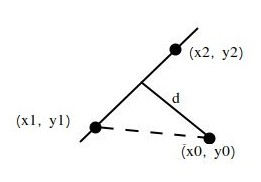
\includegraphics[width=0.5\textwidth]{dlugoscPktOdProstej}
\source{Na podstawie mathworld.wolfram.com}
\end{figure}

Wzór wyznaczający odległość punktu od prostej:

\begin{equation} \label{eq:distancePointLineal}
d = \frac{| (x_2 - x_1)(y_1 - y_0) - (x_1 - x_0)(y_2 - y_1) |}{\sqrt{(x_2 - x_1)^2 + (y_2 - y_1)^2}}
\end{equation}\newline

\begin{itemize}
\item Zmienne: x1, y1, x2, y2 oznaczają współrzędne geograficzne odpowiednio początku i końca drogi.
\item Zmienne x0, y0 oznaczają współrzędne punktu reprezentujące obiekt drogowy.
\item Zmienna d oznacza najkrótszą odleglość punktu od drogi.
\end{itemize}


\newpage
\section{Wyznaczanie współrzędnych punktu znajdującego się na drodze, odległego o n metrów od innego punktu}
\label{sec:pointCoordinatesFromAnotherPoint}

Istotnym aspektem działania algorytmu jest rozwiązanie problemu wyznaczenie współrzędnych punktu, znajdującego się na drodze, odległego o n metrów od innego punktu.  Jest to niezbędne w sytuacji, gdy np. program musi ustawić na drodze znak ograniczenia prędkości w odległosci n metrów od przejścia dla pieszych.

Do rozwiązania tego zadania, posłużyłem się własnościami trygonometrycznymi.


\begin{figure}[h]
\centering
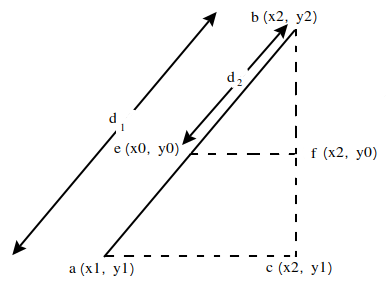
\includegraphics[width=0.5\textwidth]{distance}
\end{figure}

Odległość między dwoma punktami a i b wynosi:
\begin{equation}
d_1 = \sqrt{(x1 - x2)^2 + (y1 - y2)^2}
\end{equation}\newline

oraz sinus kąta abc:
\begin{equation}
sin_{abc} = \frac{x2 - x1}{d_1}
\end{equation}\newline

jak również sinus kąta ebf:
\begin{equation}
sin_{ebf} = \frac{x2 - x0}{d_2}
\end{equation}\newline

oraz to, że sinusy tego samego kąta są równe:
\begin{equation}
sin_{abc} = sin_{ebf} => \frac{x2 - x1}{d_1} = \frac{x2 - x0}{d_2}
\end{equation}\newline

przez proste przekształcenie, otrzymujemy wzór na współrzędną x0

\begin{equation}
x0 = x2 - \frac{d_2*(x2 - x1)}{d_1}
\end{equation}\newline

Wyznaczenie wzoru na współrzędną y0 jest podobne do wyznaczania współrzędnej x0, z tą różnicą, że zamiast sinusa, liczymy cosinusa kąta abc:

\begin{equation}
cos_{abc} = \frac{y2 - y1}{d_1}
\end{equation}\newline

oraz cosinusa kąta ebf:
\begin{equation}
cos_{ebf} = \frac{y2 - y0}{d_2}
\end{equation}\newline

a skoro cosinus tego samego kąta są równe:
\begin{equation}
cos_{abc} = cos_{ebf} => \frac{y2 - y1}{d_1} = \frac{y2 - y0}{d_2}
\end{equation}\newline

otrzymujemy równanie współrzędnej y0:
\begin{equation}
y0 = y2 - \frac{d_2*(y2 - y1)}{d_1}
\end{equation}\newline

Przez powyższe obliczenia, wyznaczone zostały wspórzędne poszukiwanego punktu:

\begin{equation} \label{eq:calculatedCoordinates}
(x2 - \frac{d_2*(x2 - x1)}{d_1}, y2 - \frac{d_2*(y2 - y1)}{d_1})
\end{equation}\newline

\newpage
\section{Wyznaczanie minimalnego obszaru pokrywającego}
\label{sec:Wyznaczanieminimalnegoobszarupokrywającego}

W niniejszej sekcji skupię się na sposobie w jaki algorytm wyznacza minimalny obszar pokrywający (eng. minimum bounding box). Będzie on wykorzystany w późniejszych obliczeniach, mających na celu przypisanie poszczególnych dróg do danych obszarów, na których obowiązuje ograniczenie prędkości.

Rys. \ref{sec:minBoundingBoxFirst} przedstawia przykładowy wielokąt reprezentujący interesujący nas obiekt pobrany z OpenStreetMap.

\begin{figure}[h]
\caption{Przykładowy wielokąt reprezentujący obiekt na mapie}
\label{sec:minBoundingBoxFirst}
\centering
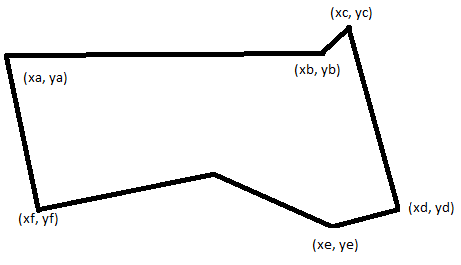
\includegraphics[width=0.8\textwidth]{minBoundingBoxFirst}
\end{figure}

W celu znalezienia minimalnego obszaru pokrywający niezbędne jest wyznaczenie czterech współrzędnych (x1, y1), (x2, y2), (x3, y3), (x4, y4) reprezentuących cztery wierzchołki prostokąta.

W celu wyznaczenia wierzchołka północno-zachodniego, należy obliczyć minimalną wartość współrzędnej x oraz maksymalną wartość współrzędnej y.

\begin{equation} \label{sec:drugiWierzcholek}
\begin{split}
x1 = min(x_a, x_b, x_c, x_d, x_e, x_f, x_g) \\
y1 = min(y_a, y_b, y_c, y_d, y_e, y_f, y_g)
\end{split}
\end{equation}\newline

Żeby wyznaczyć wierzchołek północno-wschodni, należy obliczyć maksymalną wartość współrzędnej x i y.
\begin{equation} \label{sec:trzeciWierzcholek}
\begin{split}
x2 = max(x_a, x_b, x_c, x_d, x_e, x_f, x_g)  \\
y2 = max(y_a, y_b, y_c, y_d, y_e, y_f, y_g)
\end{split}
\end{equation}\newline

Wierzchołek południowo-wschodni obliczamy jako maksymalną wartość współrzędnej x oraz minimalną wartość wsółrzędnej y.
\begin{equation} \label{sec:czwartyWierzcholek}
\begin{split}
x3 = max(x_a, x_b, x_c, x_d, x_e, x_f, x_g) \\
y3 = min(y_a, y_b, y_c, y_d, y_e, y_f, y_g)
\end{split}
\end{equation}\newline

Aby wyznaczyć południowo-zachodni wierzchołek, należy obliczyć minimalną wartość współrzędnej x i y.

\begin{equation} \label{sec:pierwszyWierzcholek}
\begin{split}
x4 = min(x_a, x_b, x_c, x_d, x_e, x_f, x_g) \\
y4 = min(y_a, y_b, y_c, y_d, y_e, y_f, y_g)
\end{split}
\end{equation}\newline

Po wyznaczeniu powyższych współrzędnych minimalny obszar pokrywający wygląda tak, jak na rysunku \ref{sec:secondtBB}


\begin{figure}[h]
\caption{Minimalny obszar pokrywający dany obiekt}
\label{sec:secondtBB}
\centering
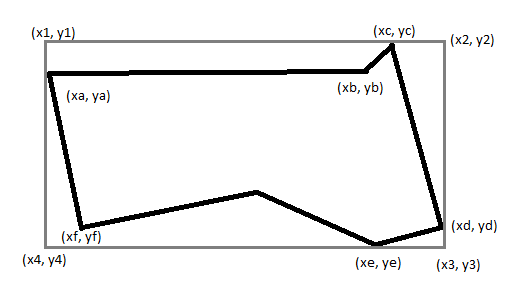
\includegraphics[width=0.9\textwidth]{minBoundingBox}
\end{figure}

\newpage
\section{Powiększanie wyznaczonego obszaru pokrywającego}
\label{sec:Powiększanie wyznaczonegoobszarupokrywającego}

Kolejnym krokiem niezbędnym do przyporządkowania dwuwymiarowych obiektów do poszczególnych dróg jest powiększenie wyznaczonego obszaru pokrywającego. W celu wyznaczenia wierzchołków powiększonego obszaru, skorzystam z poniżej podanych równań.

\begin{equation}
\begin{split}
x1' = x1 - n \\
y1' = y1 + n \\
\end{split}
\end{equation}

\begin{equation}
\begin{split}
x2' = x2 + n \\
y2' = y2 + n \\
\end{split}
\end{equation}

\begin{equation}
\begin{split}
x3' = x3 + n \\
y3' = y3 - n \\
\end{split}
\end{equation}

\begin{equation}
\begin{split}
x4' = x4 - n \\
y4' = y4 - n \\
\end{split}
\end{equation}

Rys. \ref{sec:thirdBB} przedstawia minimalny obszar pokrywający powiększony o n metrów względem pierwotnego. Oczywiście obszar można dowolnie powiększać, w zależności od obiektu, który się w nim znajduje. Tak więc dla placów zabaw czy przedszkoli będzie znacznie większy, w porównaniu do np. przystanków autobusowych.

\begin{figure}[h]
\caption{Minimalny obszar pokrywający dany obiekt powiększony o n metrów}
\label{sec:thirdBB}
\centering
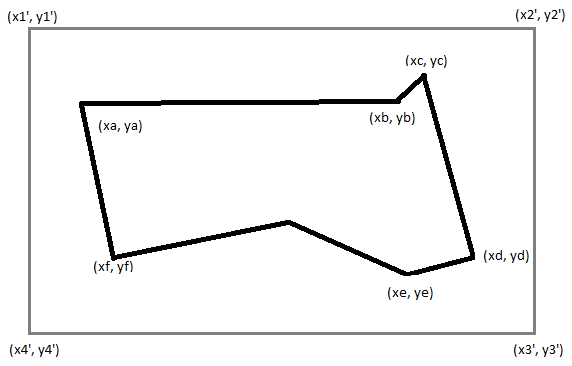
\includegraphics[width=0.7\textwidth]{BoundingBoxExtended}
\end{figure}

\newpage
\section{Łączenie powiększonych obszarów pokrywających}
\label{sec:laczeniepowiekszonychobszarwwpokrywajacych}

W celu przyszpieszenia części algorytmu odpowiedzialnego za przypisywanie danego odcinka drogi do obszaru w którym obowiązuje ograniczenie prędkości, niezbędne jest połączenie nachodzących na siebie obszarów oraz wyznaczenie jego konturu. Można rozróżnić kilka przypadków:
\begin{itemize}
\item gdy jeden obszar całkowicie znajduje się wewnątrz drugiego
\item gdy dwa rogi obszaru mającego kształt prostokątu znajdują się wewnątrz innego obszaru
\item gdy tylko jeden róg obszaru mającego kształt prostokątu znajdje się wewnątrz innego obszaru
\end{itemize}
W niniejszych podrozdziale skupię na dokładnej metodzie wyznaczania konturu dla każdego z powyższych przypadków.

\subsection{Łączenie powiększonych obszarów pokrywających w przypadku gdy jeden obszar w całości znajduje się w drugim}

Do sytuacji w której dany obszar pokrywający w całości znajduje się wewnątrz innego obszaru dochodzi gdy np. wokół przedszkola znajduje się plac zabaw. W takiej sytuacji
można pominąć wewnętrzy obszar. Na rys \ref{fig:boundingBoxInside} został przedstawiony taki przypadek.

\begin{figure}[h]
\caption{Obszar pokrywający wewnątrz innego obszaru}
\label{fig:boundingBoxInside}
\centering
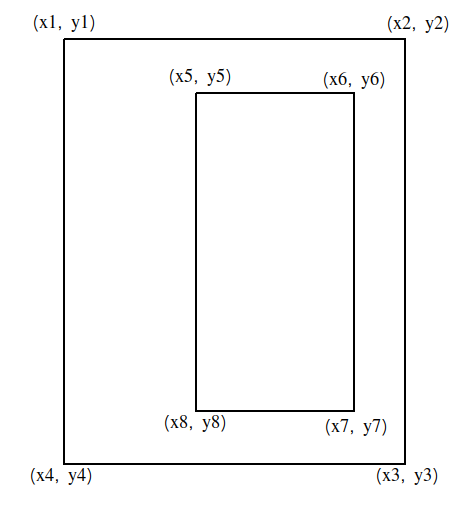
\includegraphics[width=0.6\textwidth]{boundingBoxInside}
\end{figure}

W pierwszym kroku należy znaleźć takie obszary. W tym celu algorytm iteruje po wszystkich obszarach i sprawdza, czy współrzędne spełniają wszystkie niżej przedstawione warunki.

\begin{equation}
\begin{split}
x4 <= x5 <= x2 \\
x4 <= x7 <= x2 \\
y4 <= y5 <= y2 \\
y4 <= x7 <= y2
\end{split}
\end{equation}

W następnym kroku algorytm usuwa tak znaleziony obszar. W wyniku czego na mapie pozostaje tylko obszar przestawiony na rys.\ref{fig:boundingBoxInsideRemoved}

\begin{figure}[h]
\caption{Wynik usunięcia obszaru pokrywającego wewnątrz innego obszaru}
\label{fig:boundingBoxInsideRemoved}
\centering
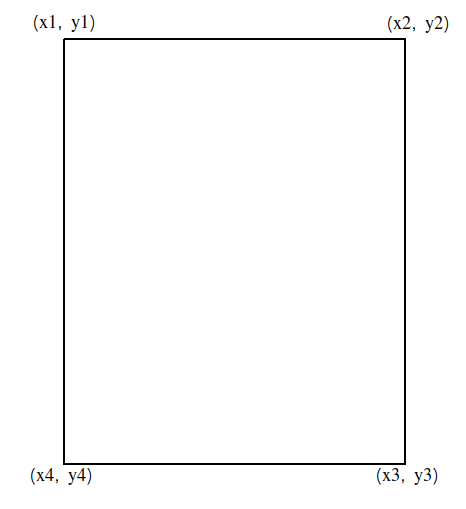
\includegraphics[width=0.6\textwidth]{boundingBoxInsideRemoved}
\end{figure}

\newpage
\subsection{Łączenie powiększonych obszarów pokrywających w przypadku gdy jeden obszar nachodzi w całości tylko jednym bokiem }

W przypadku gdy jeden obszar pokrywający w całości nachodzi tylko jednym bokiem, algorytm rozróżnia cztery możliwe sytuacje. Wszystkie one zostały przestawione na rysunku \ref{fig:OneSideBounding}.



\begin{figure}[h]
\caption{Wszystkie możliwe sytuacje w których jeden obszar nachodzi na drugi tylko jednym  bokiem}
\label{fig:OneSideBounding}
\centering
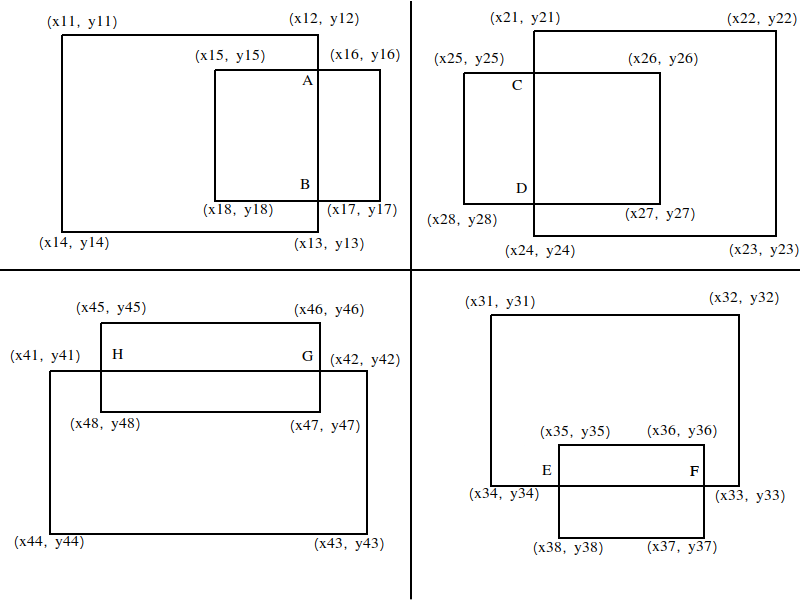
\includegraphics[width=0.8\textwidth]{OneSideBounding}
\end{figure}

W pierwszym kroku należy znaleźć takie obszary. W tym celu algorytm iteruje po wszystkich obszarach i sprawdza, czy współrzędne spełniają wszystkie niżej przedstawione warunki.

Dla pierwszej ćwiarki z rys. \ref{fig:OneSideBounding}
\begin{equation}
\begin{split}
x11 <= x15 <= x13 \\
y13 <= y15 <= y11 \\
y13 <= y18 <= y11 \\
x13 < x16 \\
\end{split}
\end{equation}

Dla drugiej ćwiarki z rys. \ref{fig:OneSideBounding}
\begin{equation}
\begin{split}
x24 <= x26 <= x22 \\
y23 <= y26 <= y21 \\
y23 <= y27 <= y21 \\
x25 < x21 \\
\end{split}
\end{equation}

Dla trzeciej ćwiarki z rys. \ref{fig:OneSideBounding}
\begin{equation}
\begin{split}
x31 <= x35 <= x33 \\
x31 <= x36 <= x33 \\
y33 <= y35 <= y11 \\
y38 < x34 \\
\end{split}
\end{equation}

Dla czwartek ćwiarki z rys. \ref{fig:OneSideBounding}
\begin{equation}
\begin{split}
x41 <= x48 <= x43 \\
x41 <= x47 <= x43 \\
y43 <= y47 <= 411 \\
y46 > x42 \\
\end{split}
\end{equation}

W następnym kroku algorytm wyznacza punkty przecięcia. Z racji tego, że nachodzące obszary są prostokątami zrotowanymi pod takim samym kątem, to do ich wyznaczenia pobiera odpowiednie współrzędne już wyznaczonych obszarów.

Dla pierwszej ćwiarki z rys. \ref{fig:OneSideBounding}

\begin{equation}
\begin{split}
A = (x12, y15) \\
B = (x12, y16)
\end{split}
\end{equation}

Dla drugiej ćwiarki z rys. \ref{fig:OneSideBounding}

\begin{equation}
\begin{split}
C = (x21, y25) \\
D = (x21, y28)
\end{split}
\end{equation}

Dla trzeciej ćwiarki z rys. \ref{fig:OneSideBounding}

\begin{equation}
\begin{split}
E = (x35, y34) \\
F = (x36, y34)
\end{split}
\end{equation}


Dla czwartej ćwiarki z rys. \ref{fig:OneSideBounding}

\begin{equation}
\begin{split}
G = (x46, y42) \\
H = (x45, y42)
\end{split}
\end{equation}

W ostatnim kroku algorytm wyznacza kontur tak przygodowanej figury, poprzez połączenie współrzędnych w odpowiedniej kolejności. Zostało to przedstawione w poniższym równaniu:

Dla pierwszej ćwiarki z rys. \ref{fig:OneSideBounding}

\begin{equation}
\begin{split}
(x11, y11) -> (x12, y12) -> (x12, y15) -> (x16, y16) ->  \\
(x17, y17) -> (x12, y16) -> (x13, y13) -> (x14, y14)
\end{split}
\end{equation}

Dla drugiej ćwiarki z rys. \ref{fig:OneSideBounding}

\begin{equation}
\begin{split}
(x21, y21) -> (x22, y22) -> (x23, y23) -> (x24, y24) ->  \\
(x21, y28) -> (x28, y28) -> (x25, y25) -> (x21, y25)
\end{split}
\end{equation}

Dla trzeciej ćwiarki z rys. \ref{fig:OneSideBounding}

\begin{equation}
\begin{split}
(x31, y31) -> (x32, 312) -> (x33, y33) -> (x36, y34) ->  \\
(x37, y37) -> (x38, y38) -> (x35, y34) -> (x34, y34)
\end{split}
\end{equation}

Dla czwartej ćwiarki z rys. \ref{fig:OneSideBounding}

\begin{equation}
\begin{split}
(x41, y41) -> (x45, y42) -> (x45, y45) -> (x46, y46) ->  \\
(x46, y42) -> (x42, y42) -> (x43, y43) -> (x44, y44)
\end{split}
\end{equation}

W wyniku powyższego algorytmu, zostały wyznaczone kontury nachodzących na siebie obszarów. Zostały przedstawione na rys. \ref{fig:OneSideBoundingRemoved}

\begin{figure}[h]
\caption{Obrys nachodzących na siebie obszarów}
\label{fig:OneSideBoundingRemoved}
\centering
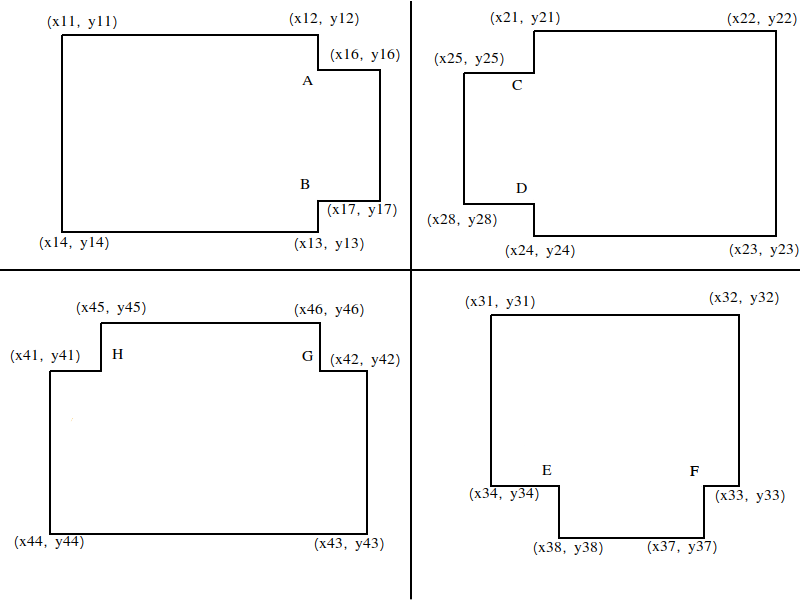
\includegraphics[width=0.75\textwidth]{OneSideBoundingRemoved}
\end{figure}

\newpage
\subsection{Łączenie powiększonych obszarów pokrywających w przypadku gdy jeden obszar nachodzi tylko jednym rogiem }

Trzecim przypadkiem nachodzenia dwóch obszarów pokrywających jest nachodzenie sie jednym rogiem. W takiej sytuacji możemy rozróżnić dwie możliwości widoczne na rys. \ref{fig:mergedKrawedzie} 

\begin{figure}[h]
\caption{Nachodzące na siebie obszary}
\label{fig:mergedKrawedzie}
\centering
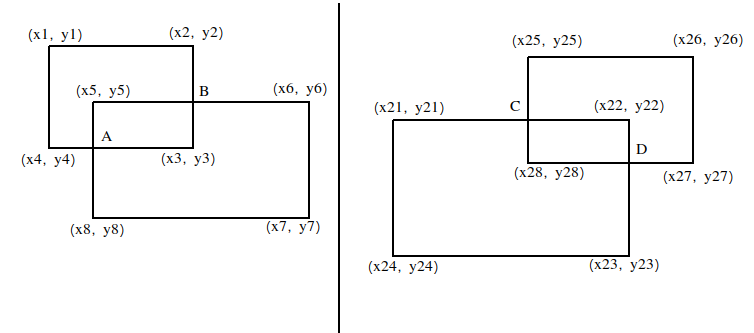
\includegraphics[width=1\textwidth]{mergedKrawedzie}
\end{figure}

W pierwszej kolejości należy znaleźć interesujące nas obszary które nachodzą na siebie. W pierwszym przypadku rys. \ref{fig:mergedKrawedzie} obszary muszą spełniać równania:

\begin{equation}
\begin{split}
x8 <= x3 <= x7 \\
y8 <= y3 <= y6 \\
x4 < x8 \\
y2 > y6
\end{split}
\end{equation}

Natomiast w drugim przypadku z rys. \ref{fig:mergedKrawedzie}:

\begin{equation}
\begin{split}
x28 <= x22 <= x27 \\
y28 <= y22 <= y25 \\
x21 < x25 \\
y23 < y28
\end{split}
\end{equation}

W następnym kroku algorytm wyznacza punkt przecięcia obu powierzchni. Z racji tego, że nachodzące obszary są prostokątami zrotowanymi pod takim samym kątem, to do ich wyznaczenia pobiera odpowiednie współrzędne już wyznaczonych obszarów. Dla pierwszego przypadku z rys. \ref{fig:mergedKrawedzie} punktu przecięcia A i B wynosi:

\begin{equation}
\begin{split}
A = (x8, y3) //
B = (x3, y6)
\end{split}
\end{equation}

Oraz dla drugiego przypadku:

\begin{equation}
\begin{split}
C = (x28, y21) //
D = (x22, y28)
\end{split}
\end{equation}

W końcowej fazie algorytm wyznacza kontur nachodzących obszarów. W pierwszym przypadku kolejność współrzędnych konturu wygląda następująco:
 
\begin{equation}
\begin{split}
(x1, y1) -> (x2, y2) -> (x3, y6) -> (x6, y6) ->  \\
(x7, y7) -> (x8, y8) -> (x8, y3) -> (x4, y4)
\end{split}
\end{equation}

A w drugim: 

\begin{equation}
\begin{split}
(x21, y21) -> (x28, y21) -> (x25, y25) -> (x26, y26) ->  \\
(x27, y27) -> (x22, y28) -> (x23, y23) -> (x24, y24)
\end{split}
\end{equation}

Wynik powyższych krókow został przestawiony na rys. \ref{fig:mergedKrawedzieKontur}

\begin{figure}[h]
\caption{Kontur nachodzących na siebie obszarów}
\label{fig:mergedKrawedzieKontur}
\centering
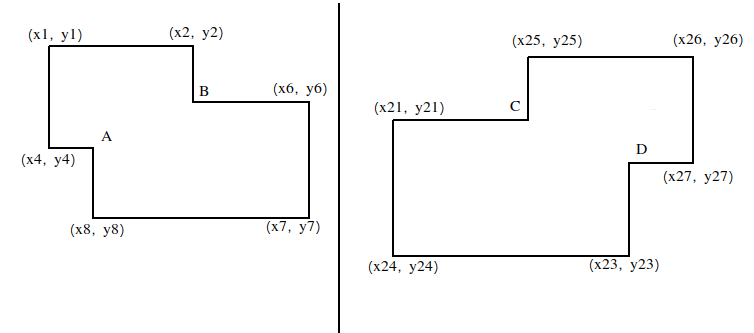
\includegraphics[width=1.1\textwidth]{mergedKrawedzieKontur}
\end{figure}

\newpage
\section{Znajdowanie punktów przecięcia drogi i powiększonego obszaru}

W celu znalezienia punktów przecięcia, wykorzystam fakt, że droga reprezentowana jest zbiór odcinków.

W pierwszej kolejności algorytm będzie iterował po zbiorze odcinków. Każdy odcinek lub bok obszaru reprezentowany jest przez dwie współrzędne:

\begin{equation}
\begin{split}
(x_a, y_a) \\
(x_b, y_b) \\
\end{split}
\end{equation}

Dzięki temu, bez problemu można określić równanie prostej przechodzącej przez te dwa punkty:

\begin{equation}
(y - y_a) (x_b-x_a) - (y_b - y_a) (x - x_a) = 0
\end{equation}

Oraz równanie w postaci kierunkowej:

\begin{equation} \label{sec:prostaKierunkowa}
y=\frac{y_a - y_b}{x_a - x_b}x + (y_a - \frac{y_a - y_b}{x_a - x_b}x_a)
\end{equation}

W celu wyznaczenia współrzędnej x punktu przecięcia wystarczy porównać oba równania:

\begin{equation}
\frac{y_c - y_d}{x_c - x_d}x + (y_c - \frac{y_c - y_d}{x_c - x_d}x_c)=\frac{y_a - y_b}{x_a - x_b}x + (y_a - \frac{y_a - y_b}{x_a - x_b}x_a)
\end{equation}

W wyniku czego otrzymujemy:

\begin{equation}
x = \frac{(y_a - \frac{y_a - y_b}{x_a - x_b}x_a) - (y_c - \frac{y_c - y_d}{x_c - x_d}x_c)}{\frac{y_c - y_d}{x_c - x_d} - \frac{y_a - y_b}{x_a - x_b}}
\end{equation}

Aby wyznaczyc współrzędną y, należy przekształcić równanie \ref{sec:prostaKierunkowa} do postaci:

\begin{equation}
x=\frac{y - (y_a - \frac{y_a - y_b}{x_a - x_b}x_a)}{\frac{y_a - y_b}{x_a - x_b}}
\end{equation}

Następnie porównać równania obu prostych:

\begin{equation}
\frac{y - (y_a - \frac{y_a - y_b}{x_a - x_b}x_a)}{\frac{y_a - y_b}{x_a - x_b}}=\frac{y - (y_c - \frac{y_c - y_d}{x_c - x_d}x_c)}{\frac{y_c - y_d}{x_c - x_d}}
\end{equation}

W wyniku czego otrzymujemy wzór na współrzędną y przecinającą obie proste:
\begin{equation}
y = \frac{(y_a - \frac{y_a - y_b}{x_a - x_b}x_a)(\frac{y_c - y_d}{x_c - x_d}) - (\frac{y_a - y_b}{x_a - x_b})(y_c - \frac{y_c - y_d}{x_c - x_d}x_c)}
{(\frac{y_c - y_d}{x_c - x_d})(\frac{y_a - y_b}{x_a - x_b})}
\end{equation}

\newpage
\section{Sprawdzanie, czy punkt przecięcia należy do odcinka}

W celu sprawdzenia, czy punkt przecięcia należy do odcinka, posłużę się własnością, że suma długości mierzonej od początku odcinka do danego punktu oraz od danego punktu, do końca odcinka jest równa całkowitej długości odcinka.

\begin{equation} \label{eq:pointInSegment}
|AC| + |CB| = |AB|
\end{equation}

W celu lepszego zobrazowania, posłuże się rysunkiem \ref{sec:pointSegment}

\begin{figure}[h]
\caption{Punkt wewnątrz odcinka}
\label{sec:pointSegment}
\centering
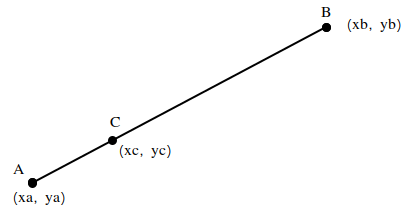
\includegraphics[width=0.8\textwidth]{pointInSegment}
\end{figure}

Odległość między dwoma punktami a i b wynosi:
\begin{equation}
d = \sqrt{(x1 - x2)^2 + (y1 - y2)^2}
\end{equation}\newline

Długość odcinka AC wynosi:

\begin{equation} \label{eq:distanceBetweenTwoPointAC}
d_{AC} = \sqrt{(xa - xc)^2 + (ya - yc)^2}
\end{equation}\newline

Długość odcinka CB wynosi:
\begin{equation} \label{eq:distanceBetweenTwoPointCB}
d_{CB} = \sqrt{(xc - xb)^2 + (yc - yb)^2}
\end{equation}\newline

Oraz długość odcinka AB wynosi:
\begin{equation}
d_{AB} = \sqrt{(xa - xb)^2 + (ya - yb)^2}
\end{equation}\newline

Zgodnie z równaniem \ref{eq:pointInSegment}, aby punkt nalezał do odcinka, musi spełniać warunek:

\begin{equation}
\sqrt{(xa - xb)^2 + (ya - yb)^2} = \sqrt{(xa - xb)^2 + (ya - yb)^2} + \sqrt{(xc - xb)^2 + (yc - yb)^2}
\end{equation}\newline


\newpage
\section{Przyporządkowanie obiektów reprezentowanych przez wielokąty, do poszczególnych dróg}
\label{sec:polygonLineDistance}

W niniejszej sekcji skupię się na rozwiązaniu problemu przyporządkowania obiektów reprezentowanych przez wielokątny do poszczególnych dróg. Wykorzystywane jest w sytuacjach, gdy trzeba określić dokładne współrzędne początku i końca strefy, na której obowiązuje ograniczonej prędkości. Obiekty na mapie, reprezentowane przez wielokąty:
\begin{itemize}
\item szkoły
\item parki
\item place zabaw
\item przystanki autobusowe i tramwajowe
\item sklepy
\item miejsca kultu
\end{itemize}


W pierwszej kolejności algorytm znajduje minimalny obszar pokrywający (eng. minimum bounding box) dany obiekt. Dokładny opis został przedstawiony w sekcji \ref{sec:Wyznaczanieminimalnegoobszarupokrywającego}

Następnie, następuje powiększenie wyznaczonego obszaru pokrywającego w celu poszerzenia strefy ograniczonej prędkości. Szczegóły znajdują się w sekcji \ref{sec:Powiększanie wyznaczonegoobszarupokrywającego}

Po wykonaniu powyższych operacji, w celu optymalizacji algorytmu, następuje łączenie nachodzących na siebie powiększonych obszarów.  Zostało dokładnie omówione w sekcji \ref{sec:laczeniepowiekszonychobszarwwpokrywajacych}


Ostatnim krokiem jest wyliczenie, które drogi znajdują się o obrębie danego obszaru. Należy zaznaczyć, że Open Street Map, w przypadku łuków czy zakrętów, przedstawia je jako zbiór odcinków. Możemy tutaj wyróżnić dwa przypadki:
\begin{itemize}
\item żaden ze zbioru odcinków nie należy do danego obszaru
\item jeden lub pewna część odcinków znajduje się w obrębie danego obszaru. W takiej sytuacji należy wyznaczyć wszystkie współrzędne przecięcia, a później określić interesujące nas fragmenty drogi.
\end{itemize}




\subsubsection{Wyznaczenie obszarów drogi znajdujących się w pobliżu danego obiektu}



\newpage
\begin{figure}[h]
\caption{Droga przebiegająca przez wybrany obszar}
\label{sec:fourthBB}
\centering
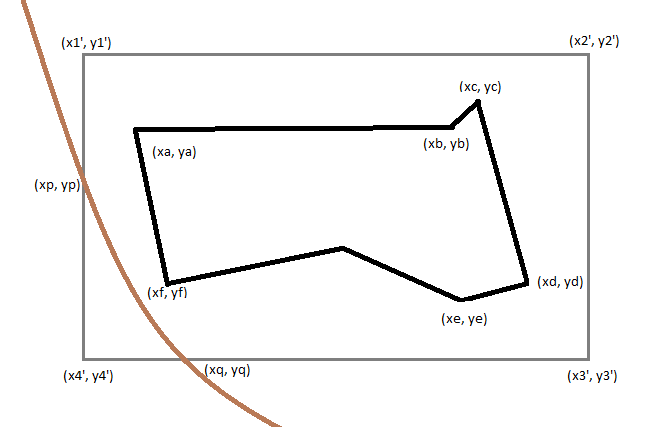
\includegraphics[width=0.8\textwidth]{minBoundingBoxWay}
\end{figure}

